\begin{figure}[b]
\centering
\textsf{
\begin{tabular}{|c|c|c|c|c|} \hline
\textbf{Year} & \textbf{Venue} & \textbf{Position} & \textbf{Event} & \textbf{Time} \\ \hline
2001 & Hungary & 2nd & 400m & 47.12 \\
2003 & Finland & 1st & 400m & 46.69 \\
2005 & Germany & 11th & 400m & 46.62 \\
2007 & Thailand & 1st & relay & 182.05 \\
2008 & China & 7th & relay & 180.32 \\ \hline
\end{tabular}
}
\\[0.5em]
\begin{tabular}{r@{ }l}
$x=$ & \runningEx \\
$z=$ & \runningLF \\
$y=$ & \{\T{Thailand}\}
\end{tabular}
\caption[
Our running example.
]{
Our running example
based on a training example from the \wtq dataset.
}\label{fig:sempre-running-ex}
\end{figure}

In the next three chapters,
we cast the task of answering a question $x$ on a web table $w$
as a \emph{semantic parsing} task.
The core idea is to model the steps for computing the answer $y$
as a compositional \emph{logical form} $z$
generated based on the input question $x$.

As a running example, consider the question
$x =$ \runningEx
on the table $w$ in Figure~\ref{fig:sempre-running-ex}.
To derive the answer \nl{Thailand},
one could identify the rows where the column \emph{Position}
contains the text \emph{1st} (2nd and 4th rows),
select the last one (4th row),
and then look for the answer in the \emph{Venue} column.
This process for computing the answer can be expressed as
the logical form
$z = \runningLF$.
(We will explain the semantics of such logical forms
in Section~\ref{sec:sempre-lf}.)
The result of executing this logical form $z$
on the table
is a \emph{denotation} $y = \set{\T{Thailand}}$,
which we use as the answer.
Using the training data,
we train our system to generate and rank logical forms $z$
so that the highest-scoring logical form
executes to the correct denotation.

Using logical forms as the intermediate representation
provides several benefits.
As logical forms are compositional and executable,
they are suitable for representing the steps needed
for answering complex questions.
Logical forms are also highly interpretable:
%unlike continuous computation states,
they explicitly show how the answer is computed.
%This is in contrast to continuous representations
%which are less interpretable
%(though continuous representations can be useful
%as the intermediate computation for generating logical forms).
Finally, the syntax and semantics of logical forms,
as well as how larger logical forms are constructed
from parts, can be customized to suit the task at hand.
In fact, we will be adapting
\emph{lambda dependency-based compositional semantics}
(lambda DCS), a formal language designed for
querying knowledge graphs \cite{liang2013lambdadcs,berant2013freebase},
to fit our task of answering questions on tables.

In this chapter, we describe our framework
for learning a semantic parser with \emph{distant supervision}:
the training dataset contains only the correct answers
and not how the answers can be derived.
We first formalize our semantic parsing framework.
We then describe the syntax and semantics of logical forms,
detailing how they can be executed on a given table.
Afterward, we explain our model that learns to parse
questions into logical forms via flexible bottom-up generation.
Finally, we report the results of our experiments
and provide analysis of our model.

\paragraph{Reference.}
The results described in this chapter have been published as
\cite{pasupat2015compositional}.
Reproducible experiments are hosted on the
CodaLab platform at
\begin{center}
\small
\url{https://worksheets.codalab.org/worksheets/0xf26cd79d4d734287868923ad1067cf4c}.
\end{center}

%%%%%%%%%%%%%%%%%%%%%%%%%%%%%%%%%%%%%%%%%%%%%%%%%%%%

\section{Framework overview}

\paragraph{Task.}
Given a table $w$ and a question $x$ about the table,
the system should produce a list $y$ of values
that answers the question.
For training, the system is given a training dataset
$\{(x\i, w\i, y\i)\}_{i=1}^N$,
where each example contains a question $x\i$,
a table $w\i$, and the correct answer $y\i$.

\begin{figure}[tp]
\centering
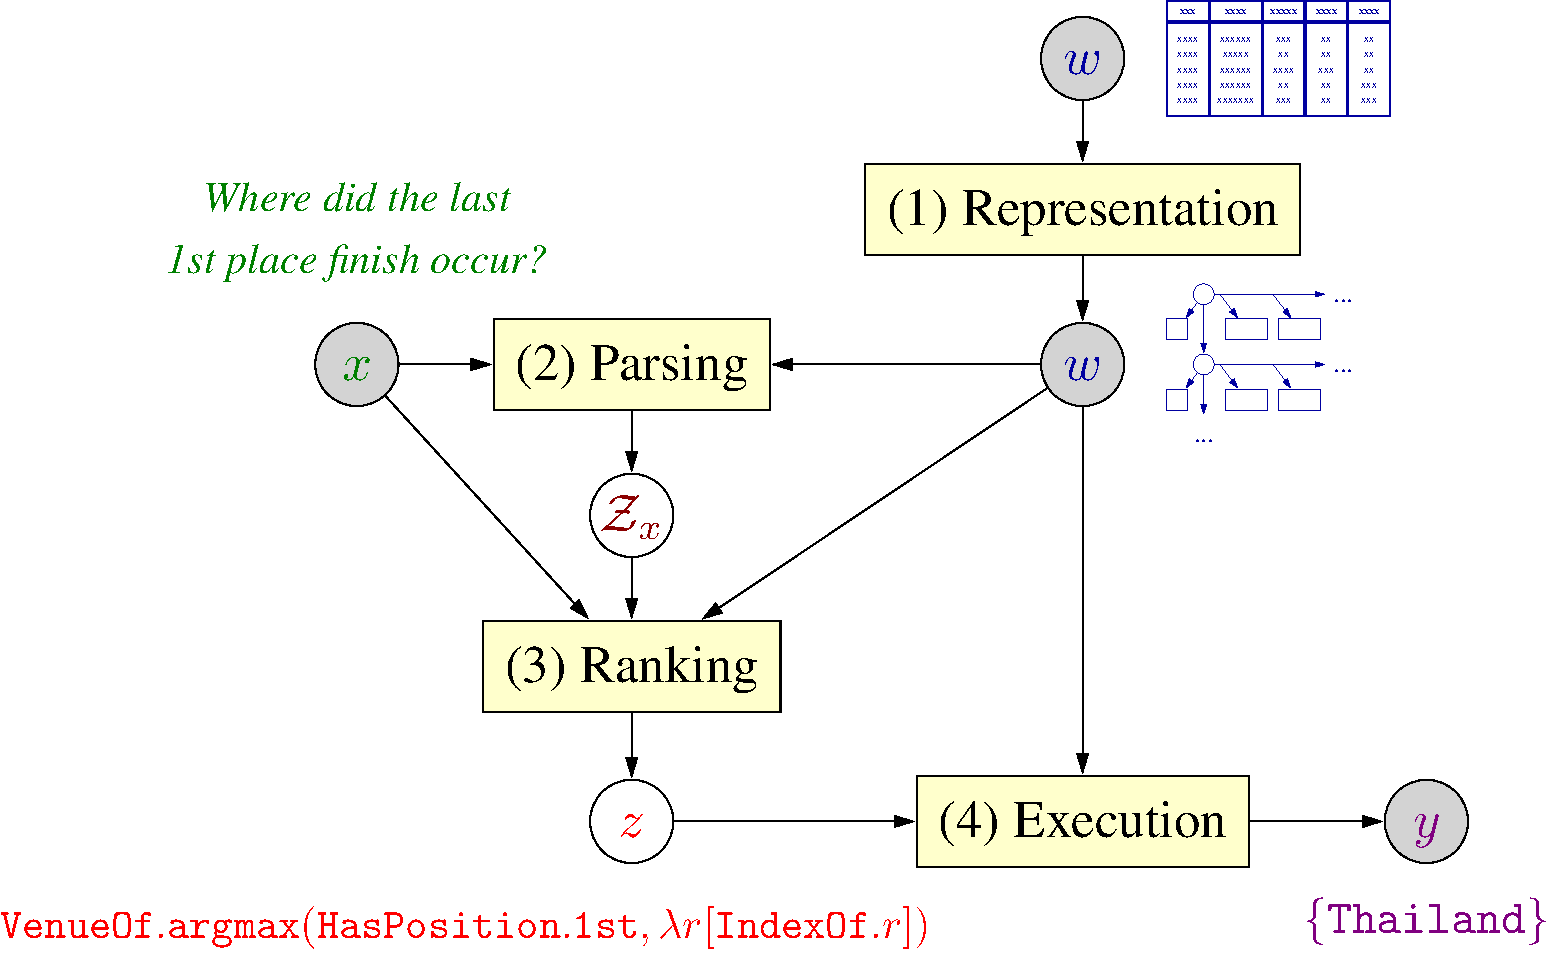
\includegraphics[scale=0.4]{sfig/sempre.slides/framework.pdf}
\caption[
The semantic parsing framework for answering questions
on web tables.
]{The semantic parsing framework for answering questions $x$
on web tables $w$.
At test time:
(1) the table $w$ is represented as a knowledge graph
as shown in Figure~\ref{fig:knowledge-graph};
(2) with information from $w$,
the question $x$ is parsed into candidate logical forms in $\zx$;
(3) the highest-scoring candidate $z\in\zx$ is chosen; and
(4) $z$ is executed on $w$, yielding the denotation $y$.
The model is trained to maximize the probability
of predicting the correct denotation.}
\label{fig:sempre-framework}
\end{figure}

\paragraph{Modeling.}
Given the question $x$ and a table $w$,
we use a logical form $z$
to represent the process for computing the answer $y$.
Formally,
we define a generative model
that generates $y$ from inputs $x$ and $w$
via a latent variable $z$.
Given a space $\Mc{Z}$ of \emph{all} possible logical forms,
we define a probability distribution
$p(z\mid x, w)$ over all $z \in \Mc{Z}$.
The probability of producing a denotation $y$ can be computed
by maginalizing over $z$:
\begin{equation}
p(y \mid x, w) =
\sum_{z \in \Mc{Z}}
\II(\deno{z}{w} = y)\,p(z \mid x, w)
\label{eqn:sempre-model}
\end{equation}
where $\deno{z}{w}$ is the denotation from executing
$z$ on $w$.

\paragraph{Prediction.}
Given a question $x$ on a table $w$,
we predict a logical form $z$ and an answer $y$
using an approximation of the generative model above.
Our prediction framework is illustrated in 
Figure~\ref{fig:sempre-framework}.
Since it is impossible to enumerate the set $\Mc{Z}$
of all possible logical forms,
we first generate a finite set of candidate logical forms
$\zx$ by parsing the question $x$ using the information
from the table $w$ (Section~\ref{sec:sempre-parsing}).
Each generated logical form $z \in \zx$
is associated with its denotation $y = \deno{x}{w}$
and a score $s_\theta(z, x, w)$,
where $s_\theta$ is a scoring function
(Section~\ref{sec:sempre-scoring})
with trainable parameters $\theta$.
We define a distribution over the candidate logical forms as
\begin{equation}
p_\theta(z \mid x, w) \propto \exp\crab{s_\theta(z, x, w)}.
\end{equation}
To predict $y$, we skip the marginalization over $z$
as written in Equation~\ref{eqn:sempre-model},
and instead just return the denotation of $z$
with the highest model probability $p_\theta(z\mid x, w)$
(or equivalently, the highest score $s_\theta(z, x, w)$).

\paragraph{Training.}
Given training data $\{(x\i, w\i, y\i)\}_{i=1}^N$,
we use a gradient ascent method to optimize $\theta$ to maximize
one of the following objective functions:

\begin{enumerate}
\item \emph{Log-likelihood of the correct denotations.}
To compute the log-likelihood of a denotation $y$,
we marginalize
over the logical forms $z \in Z_{x}$
that executes to $y$:
\begin{equation}
p_\theta(y \mid x, w) =
\sum_{z\in \zx} \II(\deno{z}{w} = y)\,p_\theta(z \mid x, w).
\end{equation}
The objective function is
\begin{equation}
J_\Mr{LL}(\theta) = 
\frac{1}{N} \sum_{i=1}^N \log p_\theta(y\i\mid x\i, w\i)
- \Omega(\theta)
\label{eqn:sempre-log-likelihood}
\end{equation}
where $\Omega$ is a regularization function.
Intuitively, a gradient update
will push up the scores of \emph{all}
consistent logical forms in $\zx$
(i.e., the ones with the correct denotation),
and push down the scores of \emph{all}
inconsistent logical forms in $\zx$.

A few previous studies have used
the log-likelihood object to train a semantic parser
\cite{kwiatkowski11lex,liang11dcs,berant2013freebase}.
While this objective function correctly maximizes
the marginalized probability of $y\i$,
it does not match the prediction process,
which does not marginalize over $z$.

\item \emph{Contrastive loss.}
From $\zx$,
we pick a logical form $z_+$
with the highest model probability among consistent
logical forms (i.e., logical forms giving the correct denotation),
and another logical form $z_-$ with the highest
probability among inconsistent logical forms.
The objective function is defined as
\begin{equation}
J_\Mr{cnt}(\theta) =
\frac{1}{N} \sum_{i=1}^N \log
\frac{p_\theta(z\i_+\mid x\i, w\i)}{p_\theta(z\i_-\mid x\i, w\i)}
- \Omega(\theta)
\end{equation}
Intuitively, a gradient update
will push up the scores of \emph{one}
consistent logical forms
and push down the scores of \emph{one}
inconsistent logical forms.
Unlike the usual contrastive loss
used in previous semantic parsing work
\cite{zettlemoyer07relaxed,zettlemoyer09context},
we always update the parameter
even when the probability of $z_+$
already exceeds that of $z_-$.
\end{enumerate}

The next four sections give more details about
each component of our framework.
Section~\ref{sec:sempre-graph} describes
how we represent the table as a \emph{knowledge graph},
which aids logical form execution and
helps us maintain uncertainty
over possible interpretations of the table.
Section~\ref{sec:sempre-lf} describes the syntax and semantics
of \emph{lambda DCS}, our logical form language.
Afterward in Section~\ref{sec:sempre-parsing},
we look at how the
set $\zx$ of candidate logical forms is generated from the input.
Finally, Section~\ref{sec:sempre-scoring}
defines the scoring function $s_\theta(z, x, w)$.

%%%%%%%%%%%%%%%%%%%%%%%%%%%%%%%%%%%%%%%%%%%%

\section{Graph representation of the table}
\label{sec:sempre-graph}

\begin{figure}[tp]
\centering
\textsf{
\begin{tabular}{|c|c|c|c|c|} \hline
\textbf{Year} & \textbf{Venue} & \textbf{Position} & \textbf{Event} & \textbf{Time} \\ \hline
2001 & Hungary & 2nd & 400m & 47.12 \\
2003 & Finland & 1st & 400m & 46.69 \\
2005 & Germany & 11th & 400m & 46.62 \\
2007 & Thailand & 1st & relay & 182.05 \\
2008 & China & 7th & relay & 180.32 \\ \hline
\end{tabular}
}
\\[1em]
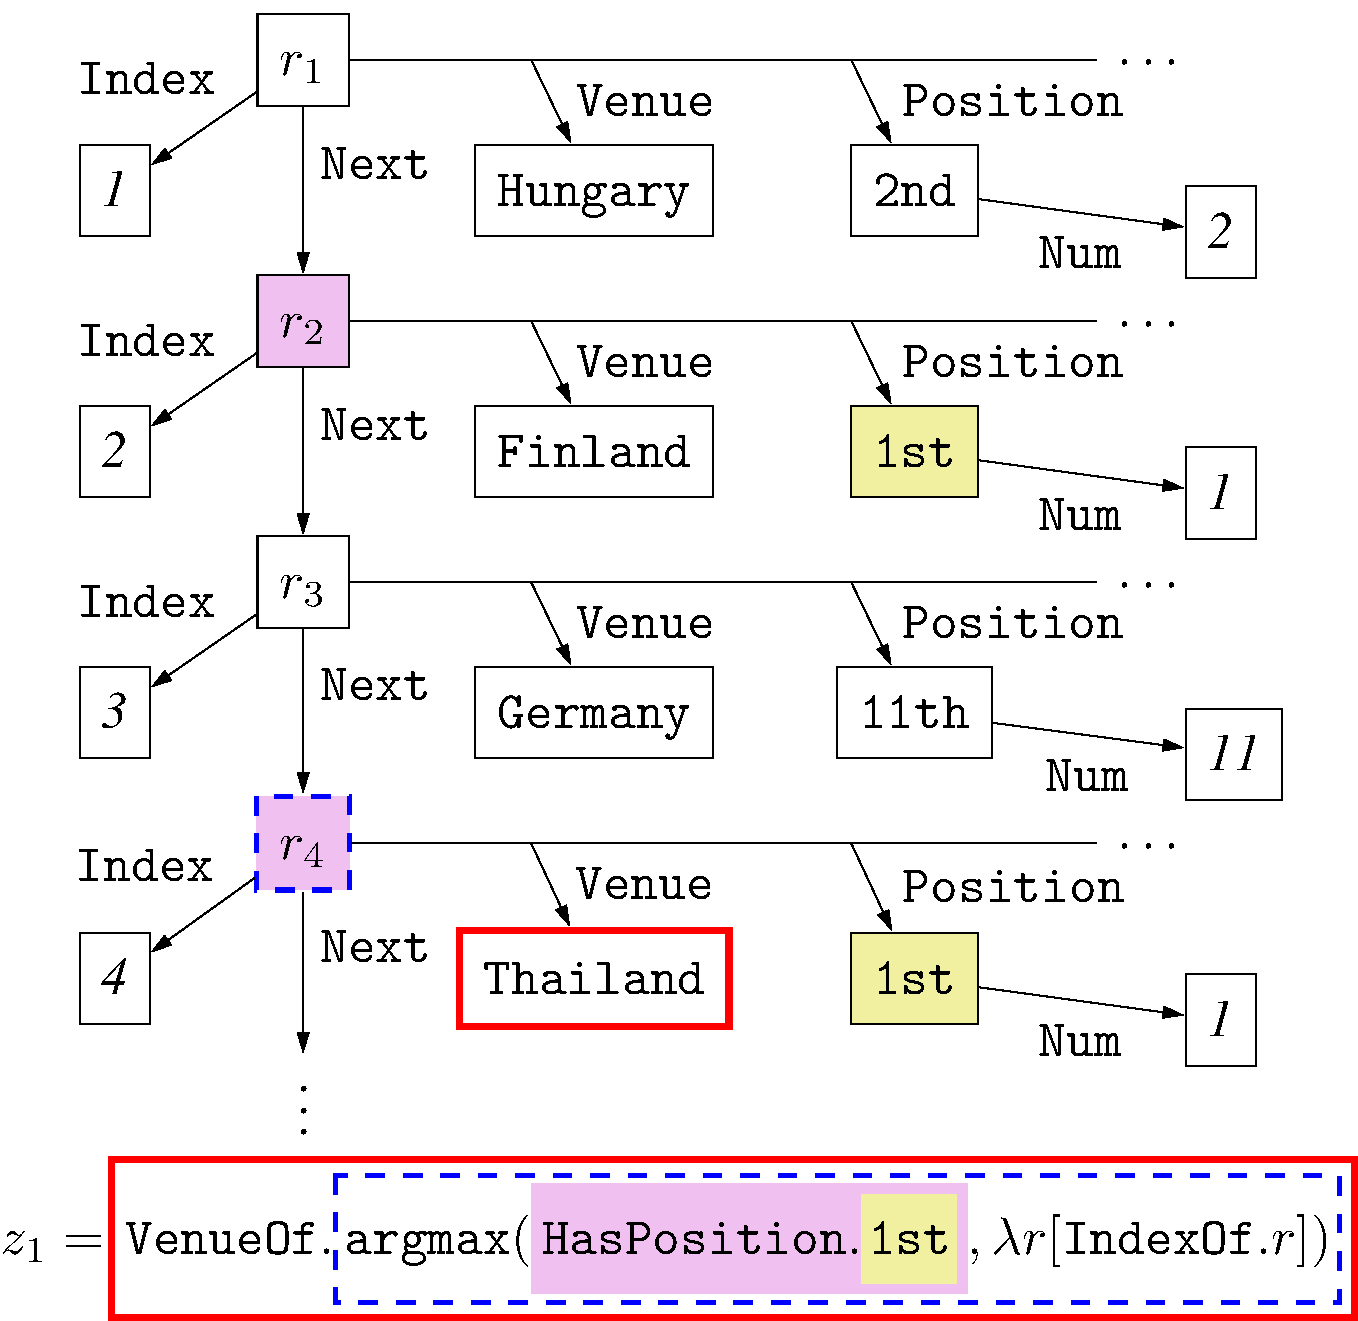
\includegraphics[scale=0.4]{sfig/dpd.slides/knowledgeGraph.pdf}
\caption[
Knowledge graph and execution of logical forms.
]{
The table $w$ is represented as a \emph{knowledge graph}.
The recursive execution of logical form $z$ is shown
via the different colors and styles.}
\label{fig:knowledge-graph}
\end{figure}

Inspired by the graph representation of knowledge bases,
we represent the table as a \emph{knowledge graph}
as illustrated in Figure~\ref{fig:knowledge-graph}.
The extensible graph structure
allows us to easily encode any additional information
by adding custom edges and nodes.
In particular, we will augment the graph with structures
for answering different types of questions
and maintaining uncertainty over different interpretations of the cell contents.

\paragraph{Basic construction.}
To construct a knowledge graph,
we first convert each row into a \emph{row node}
(e.g., the first row becomes $r_1$),
and convert cells into \emph{cell nodes}
(e.g., the cell with text \nl{Hungary}
becomes a node \T{Hungary}).
Then, we convert each column into directed \emph{column edges}
from the row nodes to the corresponding entity nodes
of that column,
and label the edges with the column header
(e.g., we construct an edge with label \T{Venue}
from $r_1$ to \T{Hungary}).
Note that columns are automatically renamed
to have unique texts if necessary.

\paragraph{Graph augmentation.}
One benefit of the graph representation
is that we can freely augment the graph with 
additional information that helps us answer the questions.

The first type of augmentation we employ is
\emph{normalization nodes}.
Some cell strings (e.g., \nl{2001})
can be interpreted as a number, a date, or a proper name
depending on the context,
while some other strings (e.g., \nl{200 km} and \nl{21-14})
have multiple parts.
Instead of committing to one normalization scheme,
we introduce normalization nodes for the possible ways
to interpret the cell strings,
and use special edges to link cell nodes to normalization nodes.
In this chapter, we consider two types of normalization:
\T{Num} (value of the first number in the cell)
and \T{Date} (year, month, and/or date that can be parsed from the cell).
For instance, a cell node \T{2001}
will have a \T{Num} edge pointing to the atomic value \C{2001.0},
and a \T{Date} edge pointing to the atomic value \C{2001-XX-XX}.

The second type of augmentation are row-specific edges.
Questions about tables usually involve reasoning about the
order of the rows. For instance,
\nl{What is the next \dots?} or \nl{Who came before \dots?}
require looking at adjacent rows,
while \nl{Who is the last \dots?} requires looking
at the last row among a group of rows.
To help answer these types of questions,
we augment each row node with an edge labeled \T{Next}
pointing to the next row node,
and an edge labeled \T{Index} pointing to the row index number
(starting from 1).

%%%%%%%%%%%%%%%%%%%%%%%%%%%%%%%%%%%%%%%%%%%%%%%

\section{Logical forms syntax and semantics}
\label{sec:sempre-lf}

\begin{table}[!p]
\centering
\begin{tabular}{lll@{}} \toprule
\textbf{Name} & \textbf{Logical form $z$} & \textbf{Denotation $\deno{z}{w}$} \\ \midrule
%
\textbf{Reverse}
& $\Mb{R}[b]$
& $\{(p, q) \mid (q, p) \in \deno{b}{w}\}$ \\
\example
& $\Mb{R}[\T{Venue}]$
& $\{(p, q) \mid q \too{Venue} p\}$ \\ \midrule
%
\textbf{Join}
& $b.u$
& $\{p \mid \exists q, q \in \deno{u}{w} \wedge (p, q) \in \deno{b}{w}\}$ \\
\addlinespace
\explainA{
\emph{Note:} To avoid confusion regarding the direction of Join,
we use the following notations when the binary $b$ is a graph edge:
$b.u$ is written as $\yHas{b}.u$, and $\Mb{R}[b].u$ is written as $\yOf{b}.u$.
} \\ \addlinespace
\example
& $\xHas{Year}.\T{2001}$
& $\{p \mid p \too{Year} \T{2001}\} = \{r_1\}$ \\
& $\xOf{Date}.\T{2001}$
& $\{p \mid \T{2001} \too{Date} p \} = \{\C{2001-XX-XX}\}$ \\
& $\xOf{Index}.\xHas{Position}.\T{1st}$
& $\{p \mid \exists q, q \too{Index} p \wedge q \too{Position} \T{1st}\}
= \{2, 4\}$ \\
& $\T{>=}.\C{4}$
& $\{p \mid p \geq 4\}$ \\ \midrule
%
\textbf{Union}
& $u_1 \sqcup u_2$
& $\{p \mid p \in \deno{u_1}{w} \vee p \in \deno{u_2}{w}\}$ \\
\example
& $\T{Finland} \sqcup \T{Hungary}$
& $\{\T{Finland}, \T{Hungary}\}$ \\ 
%
\textbf{Intersection}
& $u_1 \sqcap u_2$
& $\{p \mid p \in \deno{u_1}{w} \wedge p \in \deno{u_2}{w}\}$ \\
\example
& $\T{>=}.\C{1980} \sqcap \T{<}.\C{1990}$
& $\{p \mid 1980 \leq p < 1990\}$ \\ \midrule
%
\textbf{Aggregation}
& $A(u)$
& $\{p \mid p = A(\deno{u}{w})\}$ \\ \addlinespace
\explainA{Choices of the aggregation function $A$ include:} \\
\explainA{$\bullet$ \T{count}: number of elements in the set} \\
\explainA{$\bullet$ \T{min} and \T{max}: minimum and maximum value
(can only be used on a set of numbers or dates)} \\
\explainA{$\bullet$ \T{sum} and \T{avg}: sum and average value
(can only be used on a set of numbers)} \\ \addlinespace
\example
& $\T{count}(\xHas{Event}.\T{400m})$
& $\{p \mid p = \T{count}(\{q \mid q \too{Event} \T{400m}\})\} = \{3\}$ \\
\midrule
%
\textbf{Arithmetic}
& $\T{sub}(u_1, u_2)$
& $\{p\mid \exists q\exists q', q \in \deno{u_1}{w} \wedge q' \in \deno{u_2}{w} \wedge p = q - q'\}$ \\ \addlinespace
\explainA{For simplicity,
we only consider subtraction since other arithmetic operations are rare in our dataset.}
\\ \addlinespace
\example
& \multicolumn{2}{l}{$\T{sub}(\xOf{Index}.\xHas{Venue}.\T{China},
\xOf{Index}.\xHas{Venue}.\T{Hungary})$ \qquad $\{5 - 1\} = \{4\}$}
\\ \midrule
\textbf{Superlative}
& $\T{argmax}(u, b)$
& $\{p \mid p \in \deno{u}{w} \text{ such that for any other }
p' \in \deno{u}{w},$ \\
& \small{(\T{argmin} is defined similarly)}
& \quad$[\exists q \forall q', (q,p) \in \deno{b}{w} \wedge
(q',p') \in \deno{b}{w}
\Rightarrow q \geq q']\}$ \\ \addlinespace
\explainA{Intuitively,
the binary $b$ can be thought of as a function
mapping $p \in \deno{u}{w}$ to a set of values.
The \T{argmax} operator chooses the values $p$ that
give the maximum mapped value.}
\\ \addlinespace
\example
& $\T{allRows}$
& $\{r_1, r_2, r_3, r_4, r_5\}$ \\
& $\lambda r[\xOf{Index}.r]$
& $\{(1,r_1), (2,r_2), (3,r_3), (4,r_4), (5,r_5)\}$ \\
& $\T{argmin}(\T{allRows},
\lambda r[\xOf{Index}.r])$
& $\{r_1\}$ (giving the minimum value $1$)\\
& $\xHas{Position}.\T{1st}$ & $\{r_2, r_4\}$ \\
& \multicolumn{2}{l}{$\T{argmax}(\xHas{Position}.\T{1st}, \lambda r[\xOf{Index}.r])$ \qquad $\{r_4\}$} \\
\bottomrule
\end{tabular}

\caption[The syntax and semantics of lambda DCS logical operators.]
{The syntax and semantics of lambda DCS logical operators.
(Variables $u$ and $b$ denote a unary and a binary, respectively.
Variables $p$ and $q$ denote arbitrary values.)}
\label{tab:lambda-dcs-operators}
\end{table}

We use \emph{lambda dependency-based
compositional semantics} \cite{liang2013lambdadcs},
or \emph{lambda DCS},
as the language of our logical forms.
The language was originally designed for semantic parsing
on large knowledge graphs
\cite{berant2013freebase}.
As the context table can be converted into a knowledge graph
(Section~\ref{sec:sempre-graph}),
the lambda DCS formalism naturally transfers to our setting.

We now describe the syntax and semantics of lambda DCS constructs.
The knowledge graph in Figure~\ref{fig:knowledge-graph}
will be used as a running example.

\paragraph{Types of logical forms.}
A lambda DCS logical form is either a \emph{unary} or a \emph{binary}.
A unary represents a set of objects
(e.g., $\set{\T{Finland}, \T{Thailand}}$).
A binary represents a mapping from objects to objects,
which we will write as a set of pairs of objects
(e.g., $\set{(r_2, \T{Finland}), (r_4, \T{Thailand})}$).
We use $\deno{z}{w}$ to denote the denotation of $z$
with respect to the knowledge graph $w$
(i.e., the result of executing $z$ on $w$).

\paragraph{Primitives.}
Primitives are the smallest building blocks of lambda DCS logical forms.
Under the context of a knowledge graph $w$ from Section~\ref{sec:sempre-graph},
the primitive unaries are cell nodes
(e.g., $z = \T{Finland}$ with denotation $\deno{z}{w} = \set{\T{Finland}}$),
atomic values such as numbers and dates
(e.g., $z = \C{2001-XX-XX}$; $\deno{z}{w} = \set{\C{2001-XX-XX}}$),
and the special \T{allRows} symbol that executes
to the set of all row nodes (e.g.,
in our running example, $\deno{\T{allRows}}{w} = \{r_1, r_2, r_3, r_4, r_5\}$).

The primitive binaries are the graph edges
(e.g., $z = \T{Venue}; \deno{z}{w} = \set{(r_1, \T{Hungary}), (r_2, \T{Finland}), \dots}$)
and special binaries \T{=}, \T{!=}, \T{<}, \T{<=}, \T{>}, and \T{>=}
(e.g., $z = \T{<}$; $\deno{z}{w} = \set{(p, q) \mid p < q}$).

\paragraph{Operators.}
Larger logical forms can be constructed from smaller ones
using \emph{logical operators}.
Table~\ref{tab:lambda-dcs-operators}
lists the operators we use in our work.
Note that the direction of the binary
in our superlative operator (\T{argmax} and \T{argmin})
is the reverse of that in \citet{liang2013lambdadcs}.
This is to make the syntax more consistent
with the key-based comparison functions in many programming languages
(e.g., the logical form
$\T{argmax}(u, \lambda p[f(p)])$ is equivalent to
``\verb|max(u, key=lambda p: f(p))|'' in Python and
``\verb+u.max_by {|p| f(p)}+'' in Ruby).

\paragraph{Lambda abstraction.}
As seen in the examples of superlatives in
Table~\ref{tab:lambda-dcs-operators},
one way to construct more complex logical forms
is to use \emph{lambda abstraction}
to construct a binary.
For a logical form $f(p)$ containing a free variable $p$,
the construct $\lambda p[f(p)]$
is a binary with denotation
$\{(q, p) \mid q \in \deno{f(p)}{w} \}$.
For example, the binary
$\lambda p[\T{count}(\xHas{Event}.p)]$
counts the number of rows for each value in the \emph{Event}
column, and thus executes to
$\{(3, \T{400m}), (2, \T{Relay})\}$.\footnote{
Technically, the denotation also contains
$(0, p)$ for any other values $p$.}

\paragraph{Terminologies.}
Each token in a logical form is called a \emph{predicate}.
A logical form $z$ is \emph{consistent} with a value $y$
if its denotation $\deno{z}{w}$ matches $y$;
otherwise, it is \emph{inconsistent}.
Note that the matching can be done loosely to
get around text normalization issues
in the annotated answers
(e.g., a logical form whose denotation is $\{32\}$
is still treated as consistent with
the correct answer \nl{32 km}).

%%%%%%%%%%%%%%%%%%%%%%%%%%%%%%%%%%%%%%%%%%%%%%%

\section{Parsing the utterance into logical forms}
\label{sec:sempre-parsing}

Given a knowledge graph $w$,\footnote{
We overload the variable $w$ for both the table and
its knowledge graph representation.
Clarification will be made when necessary.}
we want to parse the input question $x$
and generate a set $\zx$ of candidate logical forms.
This section describes a bottom-up semantic parser
that produce the logical forms and their scores.

\subsection{Deduction rules}
The space of possible logical forms given the knowledge graph $w$
and the question $x$ is defined recursively
by a set of \emph{deduction rules},
which dictate how logical forms
can be constructed either from the inputs
or from smaller logical forms
\cite{zettlemoyer07relaxed,berant2013freebase}.
Informally,
our parser
maintains a set of logical forms,
and then repeatedly applies deduction rules
to construct larger logical forms
from smaller ones in the set.
Logical forms that are ``well-formed''
are finally compiled into
the set $\zx$ of candidate logical forms.
The parsing algorithm will be described more formally
in Section~\ref{sec:floating-parser}.

Deduction rules are divided into two types: terminal rules
and compositional rules.

\paragraph{Terminal rules.}
A terminal rule creates logical forms based on the input
question $x$ and knowledge graph $w$.
Each terminal rule follows one of the following templates:
\begin{align}
\C{TokenSpan}[s] &\to c[f(s)] \label{eqn:rule-b1} \\
\varnothing &\to c[f()] \label{eqn:rule-b2}
\end{align}

A rule of Template~\ref{eqn:rule-b1} takes
a token span from the question $x$
and applies the \emph{semantic function} $f$,
which generates a set of logical forms.
The resulting logical forms will be associated with
a \emph{category} $c$, which is used to enforce type consistency.
For instance, let $\mathrm{match}$ be a function
that takes a string $s$
and returns cell nodes whose cell content strings
match $s$.
Then the deduction rule
\begin{equation}
\C{TokenSpan}[s] \to \C{Entity}[\mathrm{match}(s)]
\end{equation}
can construct logical forms of category \C{Entity}
by applying the function $\mathrm{match}$
on some token span $s$ of $x$.

A rule of Template~\ref{eqn:rule-b2} works similarly,
but does not require any string from the question $x$.
Apart from generating input-independent logical forms
(e.g., \T{>=}\, and \T{allRows}),
this template is also useful when the logical form
is difficult to infer deterministically from the question.
For example, in most questions,
the relevant column names are indirectly mentioned
or implicitly implied
(e.g., the question \runningEx
in Figure~\ref{fig:sempre-running-ex}
indirectly mentions the columns \T{Venue} and \T{Position}).
We can use the following deduction rule
to generate such columns from the table:
\begin{equation}
\varnothing \to \C{Relation}[\mathrm{columns}()],
\end{equation}
where the function $\mathrm{columns}$ returns all unique column edges
from the knowledge graph $w$.

\paragraph{Compositional rules.}
A compositional rule constructs larger logical forms
from smaller ones.
Each compositional rule follows one of the following templates:
\begin{align}
c_1[z_1] &\to c[g(z_1)] \label{eqn:rule-c1} \\
c_1[z_1] + c_2[z_2] &\to c[g(z_1, z_2)] \label{eqn:rule-c2}
\end{align}

A rule of Template~\ref{eqn:rule-c1}
takes a child logical form $z_1$ of category $c$,
and then constructs a new logical form $g(z_1)$ of category $c$.
For instance, if $g(z_1) = \T{count}(z_1)$,
we can construct
$\T{count}(\xHas{Position}.\T{1st})$
from an existing logical form $\xHas{Position}.\T{1st}$.
A rule of Template~\ref{eqn:rule-c2}
operates similarly but takes two children logical forms.

\begin{table}[tb]\centering
\begin{tabular}{@{\;}r@{ $\to$ }lll@{}} \toprule
\multicolumn{2}{c}{\textbf{Rule}} & \textbf{Semantics}
& \textbf{Example} \\ \midrule

$\C{TokenSpan}$ & $\C{Entity}$
& $\mathrm{match}(s)$
& $\T{Finland}$ \\
\explainB{cell node with string $s$}
&from \emph{``Finland''} \\

$\C{TokenSpan}$ & $\C{Atomic}$
& $\mathrm{value}(s)$
& $\C{2012-07-XX}$ \\
\explainB{interpretation of $s$ at an atomic value} 
&from \emph{``July 2012''} \\

\midrule

\multicolumn{2}{l}{\quad$\varnothing$ $\to$ $\C{Relation}$}
& $\mathrm{columns}()$
& $\T{Venue}$ \\
\explainB{all column edges} \\

\multicolumn{2}{l}{\quad$\varnothing$ $\to$ $\C{Relation}$}
& $\mathrm{normalizedColumns}()$
& $\lambda x[\xHas{Year}.\xHas{Date}.x]$ \\
\explainBLong{binaries formed by joining a column edge with
a normalization edge} \\

\multicolumn{2}{l}{\quad$\varnothing$ $\to$ $\C{Records}$}
& $\T{allRows}$ \\

\multicolumn{2}{l}{\quad$\varnothing$ $\to$ $\C{RecordFn}$}
& $\lambda r.[\xOf{Index}.r]$ \\

\bottomrule

\end{tabular}
\caption[Terminal deduction rules.]{
Terminal deduction rules.
Entities and atomic values (numbers and dates) are constructed from
token spans while other predicates are not.
}\label{tab:sempre-terminal-rules}
\end{table}

%%%%%%%%%%%%%%%%%%%%%%%%%%%%%%%%%%%%%%%%%%%%%%%

\begin{table}[tb]\centering\small
\begin{tabular}{@{\;}r@{ $\to$ }lll@{\;}} \toprule
\multicolumn{2}{c}{\textbf{Rule}} & \textbf{Semantics}
& \textbf{Example} \\ \midrule

\multicolumn{4}{c}{\textbf{\emph{Join + Aggregate}}} \\ 

$\C{Entity}$ or $\C{Atomic}$ & $\C{Values}$
& $z_1$
& $\T{Finland}$ \\

$\C{Atomic}$ & $\C{Values}$
& $c.z_1$
& $\T{>=}.\C{30}$ \\
\explainB{$c \in \{\T{<}, \T{>}, \T{<=}, \T{>=}\}$} \\

$\C{Relation} + \C{Values}$ & $\C{Records}$
& $z_1.z_2$
& $\xHas{Venue}.\T{Finland}$ \\

$\C{Relation} + \C{Records}$ & $\C{Values}$
& $\Mb{R}[z_1].z_2$
& $\xOf{Year}.(\xHas{Venue}.\T{Finland})$ \\

$\C{Records}$ & $\C{Records}$
& $\xHas{Next}.z_1$
& $\xHas{Next}.(\xHas{Venue}.\T{Finland})$ \\

$\C{Records}$ & $\C{Records}$
& $\xOf{Next}.z_1$
& $\xOf{Next}.(\xHas{Venue}.\T{Finland})$ \\

$\C{Values}$ & $\C{Atomic}$
& $A(z_1)$
& $\T{count}(\xHas{Venue}.\T{Finland})$ \\
\explainB{$A \in \{\T{count}, \T{max}, \T{min}, \T{sum}, \T{avg}\}$} \\

$\C{Values}$ & $\C{ROOT}$
& $z_1$ \\

\midrule

\multicolumn{4}{c}{\textbf{\emph{Union + Intersection}}} \\

$\C{Entity} + \C{Entity}$ & $\C{Values}$
& $z_1 \sqcup z_2$
& $\T{Finland} \sqcup \T{Germany}$ \\

$\C{Records} + \C{Records}$ & $\C{Records}$
& $z_1 \sqcap z_2$
& $\xHas{Position}.\T{1st} \sqcap \xHas{Event}.\T{Relay}$ \\

\midrule

\multicolumn{4}{c}{\textbf{\emph{Superlative over rows}}} \\ 

\explainBLong{A \C{RecordFn} $\lambda r[f(r)]$
is a function that maps row nodes $r$ into comparable values} \\

$\C{Relation}$ & $\C{RecordFn}$
& $\lambda r[\Mb{R}[z_1].r]$
& $\lambda r[\xOf{Num}.\xOf{Time}.r]$ \\

$\C{Records} + \C{RecordFn}$ & $\C{Records}$
& $S(z_1, z_2)$
& $\T{argmax}(\T{allRows}, \lambda r[\xOf{Num}.\xOf{Time}.r])$ \\

\explainB{$S \in \{\T{argmax}, \T{argmin}\}$} 
& $\T{argmin}(\xHas{Position}.\T{1st}, \lambda r[\xOf{Index}.r])$ \\

\midrule

\multicolumn{4}{c}{\textbf{\emph{Arithmetic}}} \\

\explainBLong{A \C{ValueFn} $\lambda v[f(v)]$
is a function that maps values $v$ (cells or atomic values)
into comparable values} \\

$\C{Relation}$ & $\C{ValueFn}$
& $\lambda v[A(z_1.v)]$
& $\lambda v[\T{count}(\xHas{Event}.v)]$  \\

$\C{Relation} + \C{Relation}$ & $\C{ValueFn}$
& $\lambda v[\Mb{R}[z_1].z_2.v]$
& $\lambda v[\xOf{Num}.\xOf{Time}.\xHas{Event}.v]$ \\

{\scriptsize$\C{ValueFn} + \C{Values} + \C{Values}$}
& $\C{Values}$
& \hspace*{-1em}{$\T{sub}(z_1.z_2, z_1.z_3)$}
& $\T{sub}(\T{count}(\xHas{Event}.\T{400m}), \T{count}(\xHas{Event}.\T{Relay}))$ \\

\bottomrule

\end{tabular}
\caption[Compositional deduction rules.]{
Compositional deduction rules.
Each rule $c_1, \dots, c_k \to c$ takes logical forms $z_1, \dots, z_k$
constructed over categories $c_1, \dots, c_k$, respectively,
and produces a logical form based on the semantics.
}\label{tab:sempre-compositional-rules}
\end{table}

\paragraph{List of deduction rules.}
Tables~\ref{tab:sempre-terminal-rules}~and~\ref{tab:sempre-compositional-rules}
detail the deduction rules used in our parser.
The deduction rules are designed to be closely mimic
the compositional syntax of lambda DCS.
However, as some lambda DCS constructs are very generic
and can generate many nonsensical logical forms
(e.g., the subtraction operator can subtract
any two arbitrary numbers),
some operators are restricted to be applied
only in certain contexts
(e.g., only allow subtracting numbers from two cells
from the same column).
This trade-off prevents us from
answering some small number of sophisticated questions,
but we found it necessary for making the space
of generated logical forms manageable.

From the table,
we can see that many deduction rules
construct logical forms
without referencing the question.
These include the terminal rules of the form
$\varnothing \to c[f()]$
and various compositional rules
that generate operators
(e.g., \T{argmax} can be generated even when
the question does not have any word that expresses superlative).
This is intentional for two reasons:
\begin{itemize}
\item Many logical form predicates do not explicitly align
to any token from the question.
\item Even when the alignment exist, we want to learn
such an alignment from the data.
This will be achieved by the features in the scoring module
that relate logical form predicates to the tokens in the question.
\end{itemize}

\subsection{Floating parser}\label{sec:floating-parser}
To parse the question $x$ based on the deduction rules,
we propose a new parser named \emph{floating parser}
that can construct logical forms in a flexible order.

\paragraph{Chart parser.}
To understand the motivation behind the floating parser,
let us first consider a more common bottom-up parsing algorithm:
the CKY algorithm for chart parsing.

Given an input sentence $x$ with tokens $x_1, \dots, x_n$,
the algorithm constructs and stores partial parses
with category $c$
of the token span $x_{i:j} := (x_i, \dots, x_{j-1})$
in a \emph{cell} labeled $(c, i, j)$.
Being a dynamic programming algorithm,
the CKY algorithm populates the cells in the increasing order
of their span lengths $j - i$.
To construct a parse for the cell $(c, i, j)$,
we have the following choices:
\begin{itemize}
\item Apply a terminal rule of the form
\begin{equation*}
\C{TokenSpan}[s] \to c[f(s)]
\end{equation*}
on the token span $s = x_{i:j}$ to get logical forms $z \in f(s)$.
\item Apply a compositional rule of the form
\begin{equation*}
c_1[z_1] + c_2[z_2] \to c[g(z_1, z_2)]
\label{eqn:rule-c2-again}
\end{equation*}
on $z_1$ from cell $(c_1, i, k)$ and
$z_2$ from cell $(c_2, k, j)$ (for some $k \in \set{i,\dots,j-1}$)
to get a logical form $z = g(z_1, z_2)$
\item Apply a compositional rule of the form
\begin{equation*}
c_1[z_1] \to c[g(z_1)]
\end{equation*}
on another logical form $z_1$ from the same cell $(c, i, j)$
to get $z = g(z_1)$.
To avoid an infinite loop,
one can either design the deduction rules
to not have loops,
or use heuristics to detect and stop loops.
\end{itemize}

In any case, the parse is an abstract object containing
the constructed logical form $z$, plus any other metadata necessary
to score the logical form (e.g., when applying
Rule~\ref{eqn:rule-c2-again}, we can store the child parses
where $z_1$ and $z_2$ come from).
To restrict the search space to a reasonable size,
\emph{beam search} is usually employed:
the populated cells are pruned down to some
fixed number of parses that have the highest scores.
The parses in cell $(\C{ROOT}, 0, n)$
form the set $\zx$ of final logical forms.

\paragraph{Challenges.}
Chart parsing found success in syntactic parsing,
where all words end up participating in the parse,
and the parse forms a proper tree with no reordering.
In contrast, for our semantic parsing task,
the chart parser is restrictive for several reasons:
\begin{itemize}
\item
While each parse in chart parsing belongs
to some token span $x_{i:j}$,
some semantic predicates do not naturally align
to a token.
Consider the following question on a table about
Olympic games:
\begin{center}
\nl{Greece held its last Summer Olympics in which year?} \\
$\xOf{Date}.\xOf{Year}.\T{argmax}(\xHas{Country}.\T{Greece}, \lambda r[\xOf{Index}.r])$
\end{center}
While the cell node \T{Greece} can be generated from
the word \nl{Greece}, some logical form predicates
such as \T{Country} cannot be aligned to a token span.
We could potentially learn to generate the whole
$\xHas{Country}.\T{Greece}$ from \nl{Greece},
but this requires writing more custom deduction rules.
\item
Conversely, some token does not align with
a semantic predicate.
In the example above, \nl{Summer} and \nl{Olympics}
do not manifest in the logical form.
\item
Finally, the order of question tokens
and the logical form predicates
may not align well.
In the example above,
the word \nl{year} comes last,
but the predicate \T{Year} comes first.
\end{itemize}

Previous semantic parsing work
addresses the challenges above by
using a \emph{lexicon}
that maps utterance phrases
to corresponding logical form fragments
\cite{zettlemoyer07relaxed,kwiatkowski10ccg,kwiatkowski11lex,berant2013freebase}.
The lexicon can either be manually specified
or jointly learned with the parser.
However, with an open-domain knowledge source with unknown data schema,
such as a random web table,
the lexicon is unlikely to have coverage over
the unseen relations.

We instead opt for a more general solution:
we allow some predicates to be constructed from other sources
than the utterance.
The relation between the utterance and the predicate
is instead softly captured by the scoring function.
As a result, our \emph{floating parser}
can achieve a high coverage over logical forms
even for tables with unseen data schema.

\paragraph{Floating parser.}
As motivated above,
the floating parser does not require logical form predicate to
be constructed from utterance tokens.
We replace the cells $(c, i, j)$,
with \emph{floating cells} $(c, s)$,
which will store logical forms
of category $c$ that have size $s$.
The size is measured as the number of compositional rules applied
during the construction of the logical form,
and not the number of logical form predicates.

The deduction rules now operate as follows:
\begin{itemize}
\item A terminal rule of the form
\begin{equation*}
\C{TokenSpan}[s] \to c[f(s)]
\end{equation*}
constructs $z \in f(s)$ in cell $(c, 0)$.
\item A terminal rule of the form
\begin{equation*}
\varnothing \to c[f()]
\end{equation*}
constructs $z \in f()$ in cell $(c,0)$.
This allows logical form predicates to be generated
out of thin air.
\item A compositional rule of the form
\begin{equation*}
c_1[z_1] + c_2[z_2] \to c[g(z_1, z_2)]
\end{equation*}
takes $z_1$ from cell $(c_1, s_1)$ and
$z_2$ from cell $(c_2, s_2)$
to construct $z = g(z_1, z_2)$
in cell $(c, s_1 + s_2 + 1)$.
\item A compositional rule of the form
\begin{equation*}
c_1[z_1] \to c[g(z_1)]
\end{equation*}
takes $z_1$ from cell $(c_1, s_1)$ 
to construct $z = g(z_1)$ in cell $(c, s_1 + 1)$.
\end{itemize}

\begin{figure}[t]
\centering
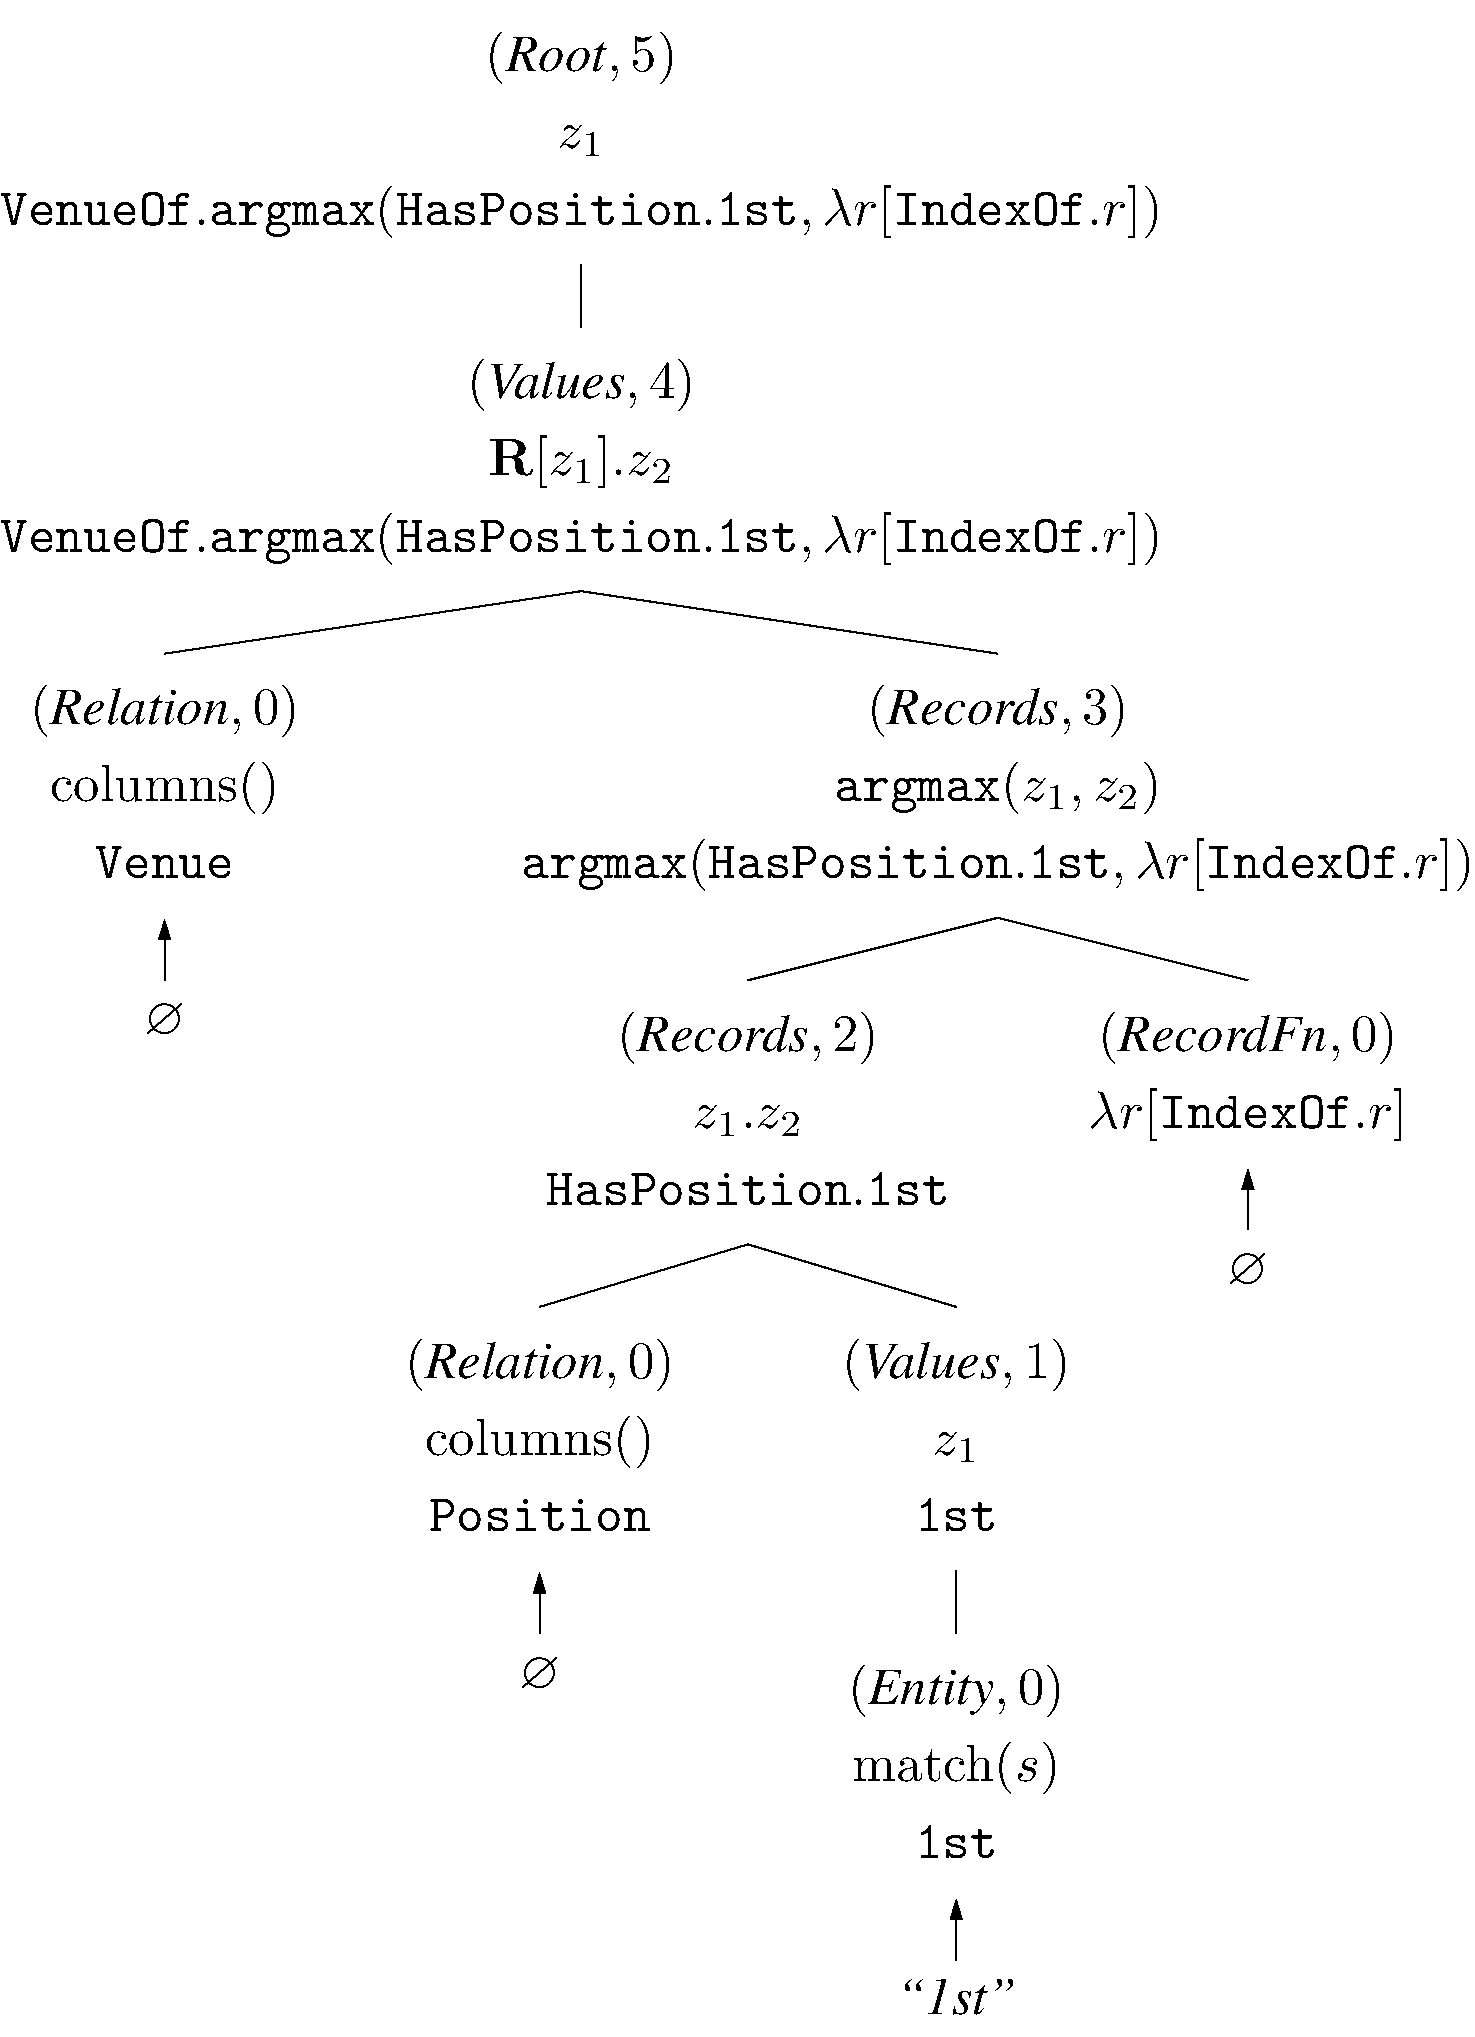
\includegraphics[scale=0.35]{sfig/parsetrees.slides/baseParse.pdf}
\caption[Derivation tree of the running example.]
{A derivation tree for the utterance \runningEx.
Each tree node shows the cell $(c,s)$,
the semantic function used,
and the resulting logical form.
Among the terminal rule applications (indicated by arrows),
only $\T{1st}$ is generated from a phrase \nl{1st} using the $\Mr{match}$ function;
other predicates are not generated based on the utterance.}
\label{fig:floating-parse-ex}
\end{figure}

Figure~\ref{fig:floating-parse-ex} shows
an example parse generated by our floating parser.
After populating the cells up to some maximum size $s = s_\Mr{max}$,
the parses in cell $(\C{ROOT}, s)$ for all sizes $s$
are compiled into the set $\zx$ of final logical forms.

\paragraph{Pruning.}

The floating parser is very flexible:
it can skip tokens,
generate tokens out of thin air,
and combine logical forms in any order.
This flexibility might seem too unconstrained,
but we can use several techniques to prevent
bad logical forms from being constructed:

\begin{itemize}
\item \textbf{Denotation-based pruning.}
Constructed logical forms can be executed
on the knowledge graph $w$ to get denotations.
We prune logical forms that execute to an empty set
(e.g., $\xHas{Year}.\xHas{Num}.\C{1}$).
While it is tempting to prune logical forms that do not execute,
care must be taken since some constructed logical forms
are partial and are meant to be used as an argument
of a larger logical form
(e.g., logical forms of category \C{ValueFn}
are meant to be used in superlative logical forms).

\begin{table} \centering
\begin{tabular}{ll} \toprule
\textbf{Criterion for pruning a logical form $z$} & \textbf{Example} \\ \midrule
% emptyDenotation + nonLambdaError
$z$ cannot be executed or executes to an empty set
& $\xHas{Venue}.\T{1st}$ \\
% forwardBackward
$z$ contains a relation joined with its inverse
& $\xOf{Position}.\xHas{Position}.\T{1st}$ \\
% doubleNext
$z$ contains a join of two $\T{Next}$ predicates
& $\xOf{Next}.\xOf{Next}.\xHas{Position}.\T{1st}$ \\
% sameMerge
$z$ is a union or intersection of identical logical forms
& $\T{1st} \sqcap \T{1st}$ \\
% mistypedMerge
$z$ is a union or intersection of values with different types
& $\T{5th} \sqcup \T{Germany}$ \\
\quad (Cells from different columns are considered different types.) \\
% badSuperlativeHead
$z$ is a superlative on a set of size 1
& $\T{argmax}(\xHas{Index}.\C{1}, \dots)$ \\
% multipleSuperlatives
$z$ contains multiple superlatives
& $\T{argmax}(\dots) \sqcap \T{argmin}(\dots)$ \\
% singleton
$z$ is a \C{ROOT} logical form with only a single predicate
& $\T{1st}$ (at category \C{ROOT})\\
% tooManyValues
$z$ is a \C{ROOT} logical form whose denotation contains > 10 values \\
\bottomrule
\end{tabular}
\caption{Heuristics for controlling the search space of the floating parser.}
\label{tab:sempre-heuristics}
\end{table}

\item \textbf{Heuristic pruning.}
Some logical forms can be properly executed,
but are unlikely to be relevant for answering the questions.
For instance, a union of objects from different columns
(e.g., $\T{5th} \sqcup \T{Germany}$)
are less likely to be reflecting what the question asks.
We use several heuristics listed in Table~\ref{tab:sempre-heuristics}
to prune logical forms.
Note that some heuristics could potentially prevent us
from answering some questions
(e.g., preventing joining two \T{Next} predicates
could prevent us from answering
\nl{What comes before the person before \dots?}).
However, these questions are rare enough,
and pruning these patterns would prune a large portion of the
search space, which increases speed and prevents overfitting
to incorrect logical form patterns.

\item \textbf{Score-based pruning (beam search).}
Even with the pruning strategies above,
the set of possible logical forms in each set
might still be large.
To control the search space,
we employ beam search by scoring the logical forms
and only keep the $B = 50$
highest-scoring logical forms in each cell.

\end{itemize}

\section{Scoring logical forms}\label{sec:sempre-scoring}

\begin{table}[t]\centering
\textsf{
\begin{tabular}{|c|c|c|c|c|} \hline
\textbf{Year} & \textbf{Venue} & \textbf{Position} & \textbf{Event} & \textbf{Time} \\ \hline
2001 & Hungary & 2nd & 400m & 47.12 \\
2003 & Finland & 1st & 400m & 46.69 \\
2005 & Germany & 11th & 400m & 46.62 \\
2007 & Thailand & 1st & relay & 182.05 \\
2008 & China & 7th & relay & 180.32 \\ \hline
\end{tabular}
} \\[.5em]
$x = \text{\nl{The last 1st place finish is in which year?}}$ \\
$z = \xOf{Num}.\xOf{Year}.\T{argmax}(\T{allRows}, \lambda r[\xOf{Index}. r])$ \\
$y = \{\C{2008}\}$
(type: \Sc{Num}, column: \T{Year}) \\[.5em]
\begin{tabular}{ll} \toprule
\textbf{Feature Name} & \textbf{Note} \\ \midrule
\textbf{phrase-predicate} \\
$\text{phrase} = \text{\nl{last}}, \text{predicate} = \T{argmax}$
& lexicalized \\
$\text{phrase} = \text{predicate}, \text{type} = \text{relation}$
& unlexicalized ($\because \text{\nl{year}} = \T{Year}$) \\
\midrule
\textbf{missing-predicate} \\
missing entity & unlexicalized ($\because$ missing \nl{1st}) \\
\midrule
\textbf{denotation} \\
$\text{denotation type} = \Sc{Num}$ \\
$\text{denotation column} = \Sc{Year}$ \\
\midrule
\textbf{phrase-denotation} \\
$\text{phrase} = \text{\nl{which year}}, \text{denotation type} = \Sc{Num}$
& lexicalized \\
$\text{phrase} = \text{denotation column}$
& unlexicalized ($\because \C{``year''} = \T{Year}$) \\
\midrule
\textbf{headword-denotation} \\
$Q = \text{\nl{which}}, \text{denotation type} = \Sc{Num}$
& lexicalized \\
$H = \text{\nl{year}}, \text{denotation type} = \Sc{Num}$
& lexicalized \\
$H = \text{denotation column}$ & unlexicalized ($\because \text{\nl{year}} = \T{Year}$) \\
\bottomrule
\end{tabular}
\caption[
Example features defined by our floating parser
]{
Example features defined
for the (incorrect) logical form $z$.
All features are binary features.
}\label{tab:features-ex}
\end{table}

Each logical form $z$ is associated with a score $s_\theta(z, x, w)$.
We adopt a linear model with features that capture the relationship
between the question $x$ and the logical form.
Concretely,
\begin{equation}
s_\theta(z, x, w) := \theta^\top \phi(z, x, w)
\end{equation}
where $\phi(z, x, w)$ is a feature vector.
Table~\ref{tab:features-ex}
shows example features from each feature type
described below:

\begin{itemize}

\item \textbf{phrase-predicate}:
For each n-gram $p_\Mr{x}$ from the question $x$
(up to 3-grams)
and a predicate $p_\Mr{z}$ from $z$,
we define a lexicalized
indicator feature
``$\text{phrase} = p_\Mr{x}, \text{predicate} = p_\Mr{z}$''.
These features capture the correspondence between
phrases and either close-classed predicates
(e.g., \nl{last} correlates with \T{argmax})
or frequent context-dependent predicates
(e.g., \nl{when} correlates with \T{Year}).

Additionally,
to handle open-domain predicates from the table,
we define an unlexicalized feature
``$\text{phrase} = \text{predicate}$''
when the phrase $p_\Mr{x}$ matches the string form of $p_\Mr{z}$.
The unlexicalized features can also have more specific details
based on substring matching,
part-of-speech tag of the phrase,
and the predicate type
(e.g., ``$\text{phrase} = \text{suffix of predicate}, \text{POS} = \text{W N}, \text{predicate type} = \text{entity}$'').

\item \textbf{missing-predicate}:
We define unlexicalized indicator features ``missing entity''
and ``missing relation''
when there are entities or relations mentioned in $x$
that are not present in $z$.

\item \textbf{denotation}:
From the denotation $y = \deno{z}{w}$,
we use its size (i.e., number of elements in the set $y$)
and its type to define unlexicalized features.
The type can be a primitive type (e.g., \Sc{Num}, \Sc{Date})
or the column containing the values in $y$
in case those values are cells.

\item \textbf{phrase-denotation}:
For each n-gram $p_\Mr{x}$ from the question $x$,
we define a lexicalized feature
``$\text{phrase} = p_\Mr{x}, \text{denotation type} = p_\Mr{y}$''
where $p_\Mr{y}$ is the type of $y$.
Like the phrase-predicate features,
we also define an unlexicalized feature
``$\text{phrase} = \text{denotation column}$''
when the type $p_\Mr{y}$ is a column whose string matches $p_\Mr{x}$.
Like phrase-predicate features, the unlexicalized feature
can be refined by substring match and part-of-speech tags.

\item \textbf{headword-denotation}:
From the part-of-speech tags of the question $x$,
we deterministically identify the question word $q_\Mr{x}$
(e.g., \emph{who}, \emph{when}, \emph{what})
and the head word $h_\Mr{x}$
(the first noun after the question word).
We then define lexicalized features
joining ``$\text{denotation type} = p_\Mr{y}$''
with ``$Q = q_\Mr{x}$'', ``$H = h_\Mr{x}$'', or both.
We also define unlexicalized features if $q_\Mr{x}$ or $h_\Mr{x}$
matches the column string of the denotation.

\end{itemize}

\section{Experiments}
We develop our model on three 80:20 splits
of the training portion of the \wtq dataset (14,152 examples),
where we report the average of three evaluation scores.
For the final evaluation,
we train on the training portion and 
test on the ``unseen'' test portion
(4,345 examples).

\subsection{Main evaluation}
The main evaluation metric is \emph{accuracy}:
the fraction of test examples where
the parser predicts the correct denotation
(in other words, the highest-ranking logical form is consistent
with the correct answer).
We also report the \emph{oracle} score:
the fraction of test examples where
the at least one of the logical forms in the
final candidate list $\zx$ is consistent with the correct answer.

\paragraph{Model details.}
We train the model using AdaGrad \cite{duchi10adagrad}
with an initial learning of 1.0.
For the experiments in this chapter,
we use the log-likelihood objective
(Equation~\ref{eqn:sempre-log-likelihood})
and lazy L1 regularization
with coefficient 0.001.
We take 3 passes over the training data.
The beam size is set to $B = 200$.

\paragraph{Baselines.}
We compare our systems to two baselines:
\begin{itemize}

\item \textbf{Information retrieval baseline (IR)}:
The IR baseline selects a cell $y$
among the table cells by applying a log-linear model
over the cells.
The features are conjunctions of the phrases of $x$
and the properties of $y$,
which covers all features of our parser
that do not depend on the logical form.

\item \textbf{\Sc{WebQuestions} baseline (WQ)}:
We restrict the logical form operators to the ones
present in the previous semantic parsing work
on the \Sc{WebQuestions} dataset
\cite{berant2013freebase}.
This includes the join and \T{count} operators.
\end{itemize}

\begin{table}[t]\centering
\begin{tabular}{lrrrr} \toprule
& \multicolumn{2}{c}{\textbf{dev}}
& \multicolumn{2}{c}{\textbf{test}} \\
\cmidrule(r){2-3} \cmidrule(l){4-5}
& \textbf{acc} & \textbf{ora} & \textbf{acc} & \textbf{ora} \\ \midrule
IR baseline & 13.4 & 69.1 & 12.7 & 70.6 \\
WQ baseline & 23.6 & 34.4 & 24.3 & 35.6 \\
Floating parser & 37.0 & 76.7 & 37.1 & 76.6 \\
\bottomrule
\end{tabular}
\caption[
Accuracy and oracles scores on
development and test data.
]{
Accuracy (acc) and oracle scores (ora) 
on the development sets
(3 random splits of the training data)
and the test data.}
\label{tab:sempre-results}
\end{table}

\paragraph{Main results.}
Table~\ref{tab:sempre-results}
shows the accuracy and oracle scores
of the floating parser and the baseline systems.
Our parser outperforms the baselines
by a significant margin.
In the following sections,
we use one of the development splits of the training data
to analyze various aspects of the \wtq dataset
and the floating parser.

\subsection{Error analysis}
\label{sec:sempre-error-analysis}

The error on the development data can be divided into the
following categories:

\paragraph{Unhandled question types (21\%).}
Due to our choices of knowledge graph representation
and logical form syntax,
some questions in the dataset cannot be answered
with logical forms.
The majority of them are:

\begin{itemize}
\item Questions with incorrect annotations.
\item Yes-no questions
(e.g., \nl{is the are of saint helena more than that of nightingale island?}).
Our logical formalism does not support boolean values.
\item Questions with the word \nl{same} or something similar
(e.g., \nl{which players played the same position as ardo kreek?}).
The answer needs to exclude the name mentioned in the question,
which is not doable with our current set of deduction rules.
\item Questions with the word \nl{consecutive} or something similar
(e.g., \nl{how many consecutive friendly competitions did chalupny score in?}).
The concept of \emph{consecutive} records cannot be computed
without augmenting the knowledge graph
(e.g., with \T{consecCompetition} values tallying the number of
consecutive repeated values so far in the \emph{Competition} column).
\end{itemize}

\paragraph{Failure to match cells (25\%).}
The cell predicates and atomic values in the logical forms
are created from two terminal rules:
\begin{align*}
\C{TokenSpan}[s] & \to \C{Entity}[\Mr{match}(s)] \\
\C{TokenSpan}[s] & \to \C{Atomic}[\Mr{value}(s)]
\end{align*}
While $\Mr{match}(s)$ uses string matching
to identify the cell from the token $s$,
sometimes the question does not use the exact string from the cell
(e.g., \nl{Italian} referring to \T{Italy},
or \nl{no zip code} referring to empty cells).
While it is possible to generate cell predicates
with a rule of the form $\varnothing \to \C{Entity}[f(s)]$
like how the column predicates are generated,
such a rule would explode the search space
as most table has a large number of cells.
On the other hand, $\Mr{value}(s)$ interprets
the utterance token span as a single cell value,
and thus cannot represent a set of multiple dates
(e.g., \nl{1980s} should match all years from 1980 to 1989).

\paragraph{Complex cell content (29\%).}
While we use normalization edges to handle different
interpretation of the cell string,
we observe several types of strings we cannot handle.
Some of these include times (e.g., \nl{1:50.81})
and multi-part strings (e.g., \nl{Belo Horizonte, Brazil},
\nl{Brazil v Germany}, or the scores \nl{7-1}).

\paragraph{Ranking errors (25\%).}
Finally, we have ranking errors
where the consistent logical form is scored lower
than the top logical form.
The most common cause is rare column names
that are not mentioned directly in the question
(e.g., \nl{airplane} not matching the column header \T{Model}).
A model that incorporates continuous word representations
could potentially reduce this type of errors.

\subsection{Ablation analysis}

\begin{table}[t]\centering
\begin{tabular}{r@{ }lrr} \toprule
&& \textbf{acc} & \textbf{ora} \\ \midrule
& \textbf{Our system} & 37.0 & 76.7 \\ 
(a) & \multicolumn{3}{l}{\textbf{Feature Ablation}} \\
& all $-$ features involving predicate & 11.8 & 74.5 \\
& \quad all $-$ phrase-predicate & 16.9 & 74.5 \\
& \qquad all $-$ lex phrase-predicate & 17.6 & 75.9 \\
& \qquad all $-$ unlex phrase-predicate & 34.3 & 76.7 \\
& \quad all $-$ missing-predicate & 35.9 & 76.7 \\
& all $-$ features involving denotation & 33.5 & 76.8 \\
& \quad all $-$ denotation & 34.3 & 76.6 \\
& \quad all $-$ phrase-denotation & 35.7 & 76.8 \\
& \quad all $-$ headword-denotation & 36.0 & 76.7 \\
(b) & \multicolumn{1}{l}{\textbf{Anchor operations to trigger words}} & 37.1 & 59.4 \\
(c) & \multicolumn{3}{l}{\textbf{Rule Ablation}} \\
& join only & 10.6 & 15.7 \\
& join + count (= WQ baseline) & 23.6 & 34.4 \\
& join + count + superlative & 30.7 & 68.6 \\
& all $-$ $\{\sqcap, \sqcup\}$ & 34.8 & 75.1 \\
\bottomrule
\end{tabular}
\caption{Average accuracy and oracle scores
on development data in various system settings.}\label{tab:sempre-ablation}
\end{table}

\paragraph{Effect of features.}
Table~\ref{tab:sempre-ablation}(a)
shows the development accuracy when a subset of features
are ablated.
The most important features are the 
lexicalized phrase-predicate features,
which learn the direct association between
words from the questions and logical form predicates
(e.g., associating \nl{last} to \T{argmax},
or associating \nl{who} with the column \T{Name}).

\begin{table}[t]\centering
\begin{tabular}{llr}\toprule
\textbf{Feature type} & \textbf{Feature} & \textbf{Weight} \\ \midrule
headword-denotation & $Q = \text{\nl{what}}, H = \text{denotation column}$ & 5.11 \\
missing-predicate & missing relation & --4.21 \\
headword-denotation & $Q = \text{\nl{which}}, H = \text{denotation column}$ & 4.09 \\
phrase-predicate & $\text{phrase} = \text{\nl{before}}, \text{predicate} = \T{<}$ & 4.07 \\
phrase-predicate & $\text{phrase} = \text{\nl{over}}, \text{predicate} = \T{>}$ & 4.02 \\
phrase-predicate & $\text{phrase} = \text{\nl{before}}, \text{predicate} = \xHas{Next}$ & 4.02 \\
headword-denotation & $Q = \text{\nl{what}}, H = \text{denotation column}, \text{denotation type} = \Sc{Date}$ & 3.74 \\
phrase-predicate & $\text{phrase} = \text{\nl{below}}, \text{predicate} = \T{<}$ & 3.72 \\
denotation & denotation is the number 0 & --3.72 \\
phrase-denotation & $\text{phrase} = \text{\nl{how}}, \text{denotation type} = \Sc{Num}$ & 3.71 \\
phrase-predicate & $\text{phrase} = \text{\nl{less}}, \text{predicate} = \T{<}$ & 3.71 \\
headword-denotation & $Q = \text{\nl{that}}, H = \text{denotation columns}$ & --3.70 \\
phrase-predicate & $\text{phrase} = \text{\nl{each}}, \text{predicate} = \T{Index}$ & --3.66 \\
custom-denotation & denotation is a negative number & --3.55 \\
phrase-predicate & $\text{phrase} = \text{\nl{last}}, \text{predicate} = \T{argmax}$ & 3.46 \\
phrase-predicate & $\text{phrase} = \text{suffix of predicate}, \text{POS} = \text{W N}, \text{predicate type} = \text{entity}$ & --3.44 \\
phrase-predicate & $\text{phrase} = \text{\nl{less than}}, \text{predicate} = \T{<}$ & 3.38 \\
headword-denotation & $Q = \text{\nl{what}}, H = \text{\nl{number}}, \text{denotation type} = \Sc{Num}$& 3.36 \\
phrase-denotation & $\text{phrase} = \text{\nl{many}}, \text{denotation type} = \Sc{Num}$ & 3.34 \\
headword-denotation & $Q = \text{\nl{how many}}, \text{denotation type} = \Sc{Num}$ & 3.32 \\
phrase-predicate & $\text{phrase} = \text{\nl{when}}, \text{predicate} = \xOf{Date}$ & 3.25 \\
phrase-predicate & $\text{phrase} = \text{\nl{team do}}, \text{predicate} = \T{Index}$ & 3.18 \\
phrase-denotation & $\text{phrase} = \text{\nl{how many}}, \text{denotation type} = \Sc{Num}$ & 3.17 \\
phrase-predicate & $\text{phrase} = \text{\nl{list before}}, \text{predicate} = \xHas{Next}$ & 3.17 \\
phrase-predicate & $\text{phrase} = \text{\nl{under}}, \text{predicate} = \T{<}$ & 3.12 \\
phrase-predicate & $\text{phrase} = \text{\nl{after}}, \text{predicate} = \xOf{Next}$ & 3.08 \\
phrase-predicate & $\text{phrase} = \text{\nl{previous}}, \text{predicate} = \xHas{Next}$ & 3.07 \\
phrase-predicate & $\text{phrase} = \text{\nl{after}}, \text{predicate} = \T{>}$ & 3.05 \\
phrase-predicate & $\text{phrase} = \text{\nl{from}}, \text{predicate} = \xOf{Date}$ & --3.03 \\
phrase-predicate & $\text{phrase} = \text{\nl{the top}}, \text{predicate} = \T{<=}$ & 3.00 \\
\bottomrule
\end{tabular}

\caption[
Top features from the parser]{
The top 30 features when sorted by the magnitude of the parameter weights.
($Q$ = question word; $H$ = headword)
}
\label{tab:sempre-best-features}
\end{table}

Table~\ref{tab:sempre-best-features}
shows the features whose parameter weights have high magnitude.
We observe that the model indeed learns to associate
question phrases with either built-in logical predicates
or common column names.
It also learns some biases in the dataset;
for instance, a numerical answer is less likely to be zero or negative.

\begin{table}[t] \centering
\begin{tabular}{cl} \toprule
\textbf{Predicate} & \textbf{Triggers} \\ \midrule
$\sqcup$ & and, or \\
$\T{Next}$ & next, previous, after, before, above, below \\
$\T{>}, \T{>=}$ & than, more, least, above, after \\
$\T{<}, \T{<=}$ & than, less, most, below, before \\
$\T{count}$ & how, many, total, number \\
$\T{sum}$ & all, combine, total \\
$\T{avg}$ & average \\
$\T{sub}$ & difference, between, and, much \\
$\T{argmax}, \T{argmin}$ & top, first, bottom, last, \emph{any word with part-of-speech tag JJR, JJS, RBR, or RBS}
\\ \bottomrule
\end{tabular}
\caption[Trigger phrases for testing if the model associates operators with tokens.]
{To test whether the model learns to associate
logical operators with tokens,
we perform an experiment where some logical forms
predicates must be explicitly triggered
by some predefined phrases.}
\label{tab:sempre-trigger-phrases}
\end{table}

\paragraph{Associating operators with tokens.}
In our floating parser,
built-in edges (e.g., \T{Index}, \T{Next}, \T{Num})
and logical operators (e.g., \T{count}, \T{argmax})
are not generated based on the question tokens,
but the model ends up learning the association
from these predicates to the tokens.
As an experiment,
we consider an alternative approach where
these predicates are explicitly generated based on
some set of ``trigger'' phrases.
Based on the training data,
we manually specify the trigger phrases
for some logical predicates
as listed in Table~\ref{tab:sempre-trigger-phrases}.
We then change the deduction rules so that
the predicates can be constructed
only when one of the phrases is present in the question.

As an explicit prior,
the trigger words help decrease the number of
generated logical forms
(before pruning to beam size).
However, the result in Table~\ref{tab:sempre-ablation}(b)
shows that trigger words
do not significantly affect the accuracy,
suggesting that our floating parser
can successfully learn the association
between phrases and logical operators
without requiring a lexicon.

\begin{figure}[t]
\centering
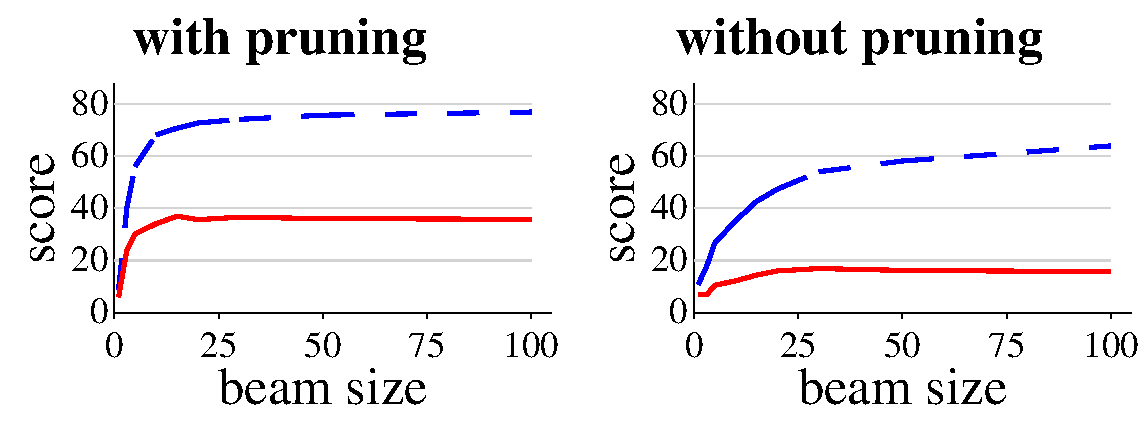
\includegraphics[scale=0.5]{sfig/sempre.slides/newBeamPlot.pdf}
\caption{
Accuracy (solid red) and oracle (dashed blue) scores with different beam sizes.
}
\label{fig:sempre-beam}
\end{figure}

\paragraph{Effect of beam size.}
Figure~\ref{fig:sempre-beam}
shows the accuracy and oracle scores
as the beam size changes.
A lower beam size increases efficiency
and prevents bad logical forms from clogging up the beam,
but when the beam size gets too low,
the accuracy and oracle scores decrease.

\subsection{Additional dataset analysis}
\label{sec:wtq-analysis-again}

Using the trained parser,
we continue our investigation from
Section~\ref{sec:wtq-analysis}
and empirically analyze several aspects of the
\wtq dataset.
% From Table~\ref{tab:sempre-results},
% our parser successfully finds a logical form
% consistent with the correct denotations in
% 76.7\% of the development examples.
% We use these consistent logical forms
% to examine the complexity of our dataset.

\paragraph{Logical form coverage.}
The \wtq dataset contains various types of reasoning
to answer the questions.
Table~\ref{tab:sempre-ablation}(c) shows the drop in accuracy
and oracle scores
when only a subset of deduction rules are allowed.
The \emph{join only} subset corresponds to table lookup,
while the \emph{join + count} subset covers the same scope
of logical forms as the previous work on the \Sc{WebQuestions} dataset
\cite{berant2013freebase}.
Finally, the \emph{join + count + superlative} subset
roughly corresponds to the coverage of the \Sc{GeoQuery} dataset \cite{zelle96geoquery}.

\begin{figure}[t]
\centering
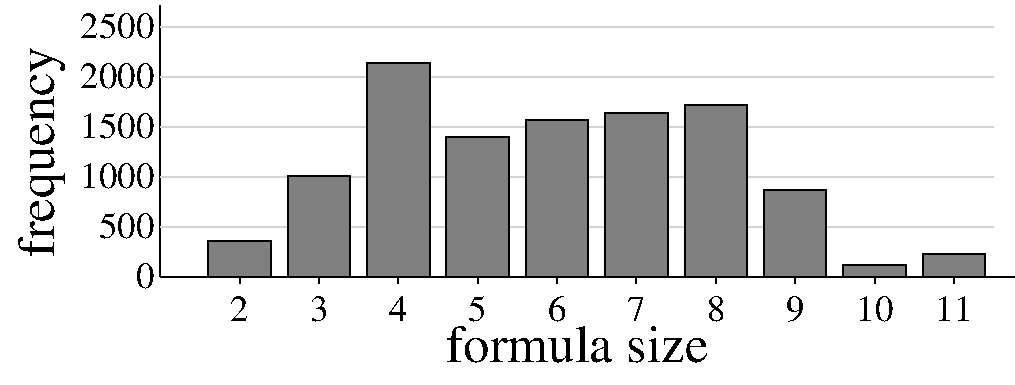
\includegraphics[scale=0.45]{sfig/sempre.slides/predCountHistogram.pdf}
\caption{
Sizes of the highest-scoring correct candidate logical forms in development examples.
}
\label{fig:sempre-lf-size}
\end{figure}

\paragraph{Compositionality.}
The histogram in Figure~\ref{fig:sempre-lf-size}
tracks the size of the logical forms
(as the number of compositional deduction rules)
that are consistent with the correct answer.
If there are consistent multiple logical forms in
the candidate set $\zx$, we choose the shortest one.
The histogram shows that a significant number of logical forms
have non-trivial sizes.

\subsection{True oracle score}
\label{sec:sempre-true-oracle}

From Table~\ref{tab:sempre-results},
our parser successfully generates a logical form
consistent with the correct denotations 
(but may or may not be the highest-scoring logical form)
in 76.7\% of the development examples.
Based on
the large gap between the accuracy (37.0\%) and this number,
one might believe that the accuracy can be improved
mainly with a better scoring model.
Unfortunately, the oracle score is misleading
due to the existence of \emph{spurious logical forms}
that give the right answer for wrong reasons.
For instance, in our running example (Figure~\ref{fig:sempre-running-ex}),
consider the spurious logical form
\begin{equation}
\xOf{Venue}.\T{argmax}(\xHas{Position}.\T{1st},
\lambda r[\xOf{Num}.\xOf{Time}.r]).
\end{equation}
From $\deno{\xHas{Position}.\T{1st}}{w} = \{r_2, r_4\}$,
the logical form picks the row with the highest \emph{Time}
instead of the highest index,
but eventually arrives at the 
correct denotation $\{\T{Thailand}\}$.
We found that in many examples,
the parser only found spurious logical forms
and not a semantically correct one.

To measure the true oracle score,
we sample 300 examples and manually annotate them
with semantically correct logical forms,
and see if the trained system can generate
the annotated logical form as a candidate.\footnote{
This method ignores generated logical forms
that are semantically
equivalent to the annotated logical forms.
Chapter~\ref{chp:dpd} will present
a more precise method that takes
logical form equivalency into account.
}
Out of 300 examples,
we find that 84\% can be manually annotated,
while the rest are unhandled questions
as explained in Section~\ref{sec:sempre-error-analysis}.

The system successfully generates the annotated
logical forms in only 53.5\% of the examples.
This indicates that the main method to improve the parser
is to increase the \emph{coverage} over answerable questions,
such as by augmenting the knowledge graph
and expanding deduction rules.
We will explore this direction of increasing coverage,
along with the efficiency problem it entails,
in the next chapter.

\section{Related work and discussion}

\paragraph{Logical form generation.}
Apart from the bottom-up generation used in our floating parser,
previous work has modelled the process of generating logical forms
with various paradigms.

Like the logical form structure,
the syntactic parse of a sentence is also hierarchical.
As such, previous work has considered using
syntactic structures to guide
the generation of semantic parses.
For instance, some take the syntactic parse
from an external parser and convert it into a semantic parse
\cite{poon2013gusp,reddy2016transforming}.
Others learn a joint model for syntactic and semantic parses.
One popular example is the use of
Combinatory Categorial Grammar
\cite{steedman1996surface,steedman00ccg}, or CCG,
which can capture syntax and semantics jointly
\cite{zettlemoyer05ccg,zettlemoyer07relaxed,kwiatkowski10ccg,kwiatkowski11lex}.

Without using syntactic structures,
one can also learn to decode the semantic parse directly.
We follow the line of work that uses
bottom-up generation
\cite{berant2013freebase,berant2014paraphrasing,berant2015agenda}.
One benefit of bottom-up generation is that
the intermediate parses are complete logical forms
that can be executed,
and the resulting denotations
can be used to prune unpromising logical forms
\cite{wang2018robust}
or as additional information
to the scoring model
\cite{guu2017bridging}.

Early \emph{neural} semantic parsing approaches
treat logical form generation as a sequence prediction problem
and just generate the predicates from left to right
\cite{jia2016recombination}.
This works well for generating canned idiomatic expressions,
but the resulting sequences are not guaranteed to be valid logical forms.
A popular alternative is top-down generation,
where at each recursion step,
the parser first selects an operator
and then recursively builds the arguments as child subtrees
\cite{dong2016logical,krishnamurthy2017neural,rabinovich2017abstract,cheng2017learning}.
One benefit of the top-down approach is that the information
from the parent node is properly propagated
to the corresponding children subtrees,
even when the subtree is generated many steps after the parent operator
is generated.

\paragraph{Hard mapping versus soft mapping.}

Early semantic parsing work assumes a strict mapping
between words in the utterance and predicates
in the logical forms.
This mapping is often called a \emph{lexicon},
which could be hand-specified
\cite{zelle96geoquery,unger2011pythia,unger2012template},
learned separately from the data
\cite{cai2013large,berant2013freebase},
or learned jointly while training the parser
\cite{zettlemoyer07relaxed,kwiatkowski10ccg,kwiatkowski11lex}.
While this works well for a specific domain,
learning such a lexicon for open-domain knowledge sources
is difficult due to the open set of phrases and predicates.
Previous work addressed this using factorized lexicon
\cite{kwiatkowski11lex}
or by translating the lexicon output to match the target
domain on the fly
\cite{kwiatkowski2013scaling}.

Our floating parser takes a similar approach to
the free-form generation of logical forms
in \citet{berant2014paraphrasing}.
Instead of a strict mapping,
we try out different logical form predicates and
uses the scorer to rank them.
This idea of soft mapping
has become the norm in neural-based parsers
\cite{jia2016recombination,dong2016logical,krishnamurthy2017neural},
where the generation of each predicate
is guided by the
embedding of the input,
while the attention mechanism \cite{bahdanau2015neural,luong2015translation}
is used as a soft alignment
between certain utterance tokens
and the generated logical predicate.
Open-domain predicates
(e.g., column and cell nodes in our case)
are generated using explicit copy mechanism
\cite{gu2016copying,jia2016recombination},
which plays a similar role to our terminal rules.

\paragraph{Table normalization.}
One challenge with working on web tables is that
the table format is not standardized.
This is surprisingly severe on Wikipedia:
while there are some general guidelines,
Wikipedia editors end up using
the most suitable table format for each article.

One way to handle the different table formats
is to convert them into canonical formats.
For instance, different table formatting can be canonicalized
to database-like formats
\cite{embley2016converting}.
Entities in the table can be linked to canonical entities
in some structured knowledge source
\cite{limaye2010annotating,bhagavatula2015tabel}.
Numerical cells can be parsed into the correct
values and units
\cite{madaan2016numerical}.
And missing data can be inferred
from an aggregation of multiple tables
\cite{venetis2011recovering}.
The canonicalization makes it easier
to perform computation on the data,
but it requires designing a good canonical schema.
Moreover, the conversion process is noisy
and might introduce errors for ambiguous cell contents.
For instance, the string
\nl{1990} is usually tagged as a date by a
named entity recognition (NER) tagger,
but could be a plain number
or a proper noun in some contexts.

Another way to handle tables
is to extract just the necessary information from the table
\cite{govindaraju2013understanding,zhang2015deepdive}.
The extracted information,
usually a relation between two entities,
can then be used to populate a database
with a known schema
\cite{ellis2015tackbp}.
Apart from having clean data suitable for computation,
this type of extraction also
allows the information from both structured data
and unstructured text to be unified and reasoned on jointly.
However,
it precludes the use of other data
available in the table that were not extracted.

Our approach is to maintain uncertainty in
table interpretation via normalization edges,
and then let the scorer
choose the correct
% The scorer is then responsible for choosing the correct
form of normalization.
This process prevents the loss of information
due to extraction.
Moreover, additional ways to interpret the cells
can be added dynamically,
as we will explore in Chapters~\ref{chp:macro}~and~\ref{chp:dpd}.
However, this also increase the search space of logical forms,
which is sometimes wasteful when the column
is clearly of a particular type.
For instance, the cell with text \emph{1990} is very likely to be a year
if all other cells also look like a year,
and keeping around the possible \T{Num} interpretation
wastefully expands the space of possible logical forms.

\section{Conclusion}
In this chapter,
we presented a semantic parsing approach for
the task of answering complex question on web tables.
To handle open-domain tables with unknown schemata,
we (1) use knowledge graph as a domain-generic representation
of the tables,
and (2) use a floating parser that can flexibly
generate logical form predicates based on the table schema.
The scoring function is then responsible for
relating the question to the generated logical forms.

To train the model with the correct answers as distant supervision,
we need to generate a set of candidate logical forms
and up-weight the ones that are consistent with the annotated answers.
Unfortunately, with more complex questions,
the space of possible logical forms rapidly expands
with the number of reasoning steps and logical operators.
This makes it expensive to generate a set of candidates
that contain a consistent logical form.
In the next two chapters, we will look at techniques
to control the search space of logical forms.
